\documentclass[12pt, a4paper]{article}

% ── Codificação e língua ──────────────────────────────────────────────
\usepackage[utf8]{inputenc}
\usepackage[T1]{fontenc}
\usepackage[brazil]{babel}

% ── Layout ───────────────────────────────────────────────────────────
\usepackage[a4paper, top=3cm, bottom=2cm, left=3cm, right=2cm]{geometry}
\usepackage{setspace}
\onehalfspacing
\usepackage{indentfirst}
\setlength{\parindent}{1.25cm}

% ── Fontes e tipografia ───────────────────────────────────────────────
\usepackage{lmodern}
\usepackage{microtype}

% ── Tabelas ──────────────────────────────────────────────────────────
\usepackage{booktabs}
\usepackage{longtable}
\usepackage{array}
\usepackage{tabularx}
\usepackage{multirow}
\usepackage{xcolor}
\usepackage{colortbl}

% ── Imagens ──────────────────────────────────────────────────────────
\usepackage{graphicx}
\usepackage{float}
\usepackage{caption}
\usepackage{subcaption}

% ── Matemática ───────────────────────────────────────────────────────
\usepackage{amsmath}
\usepackage{amssymb}

% ── Código ───────────────────────────────────────────────────────────
\usepackage{listings}
\usepackage{listingsutf8}
\lstset{
  basicstyle=\ttfamily\small,
  breaklines=true,
  frame=single,
  backgroundcolor=\color{gray!10},
  rulecolor=\color{gray!40},
  keywordstyle=\color{blue!70!black}\bfseries,
  commentstyle=\color{green!50!black},
  stringstyle=\color{red!60!black},
  numbers=left,
  numberstyle=\tiny\color{gray},
  numbersep=8pt,
  captionpos=b,
}

% ── Links e referências ───────────────────────────────────────────────
\usepackage[hidelinks]{hyperref}
\usepackage{url}

% ── Cores customizadas ────────────────────────────────────────────────
\definecolor{helmblue}{RGB}{55, 138, 221}
\definecolor{helmgreen}{RGB}{29, 158, 117}
\definecolor{helmamber}{RGB}{239, 159, 39}
\definecolor{helmred}{RGB}{226, 75, 74}
\definecolor{rowgray}{RGB}{245, 245, 243}
\definecolor{headerblue}{RGB}{220, 235, 250}
\definecolor{headergreen}{RGB}{220, 245, 235}

% ── Cabeçalho e rodapé ───────────────────────────────────────────────
\usepackage{fancyhdr}
\pagestyle{fancy}
\fancyhf{}
\fancyhead[L]{\small Helmsman — Fuzzy Auto-Scaler for Docker Web Services}
\fancyhead[R]{\small Inteligência Artificial e Computacional}
\fancyfoot[C]{\thepage}
\renewcommand{\headrulewidth}{0.4pt}

% ── Sumário ──────────────────────────────────────────────────────────
\usepackage{tocloft}

% ─────────────────────────────────────────────────────────────────────
\begin{document}

% ══════════════════════════════════════════════════════════════════════
% CAPA
% ══════════════════════════════════════════════════════════════════════
\begin{titlepage}
  \thispagestyle{empty}
  \centering

  \vspace*{1.5cm}
  {\Large \textbf{CESUPA — Centro Universitário do Estado do Pará}}\\[0.5cm]
  {\large Inteligência Artificial e Computacional}\\[0.2cm]
  {\large Prof. Daniel Leal Souza \hspace{1cm} Turma: CC5NA \hspace{1cm} Semestre: 01/2026}

  \vspace{3cm}
  \rule{\linewidth}{0.5pt}\\[0.5cm]
  {\LARGE \textbf{Helmsman}}\\[0.4cm]
  {\Large Fuzzy Auto-Scaler for Docker Web Services}\\[0.3cm]
  {\large com modo Algoritmo Genético integrado}\\[0.5cm]
  \rule{\linewidth}{0.5pt}

  \vspace{3cm}
  \begin{tabular}{l}
    Andrey de Matos Gonçalves \\[0.3cm]
    Felipe Gabriel Souza Libório \\[0.3cm]
    Felipe Vieira Brazão e Silva \\[0.3cm]
    Gabriel Coelho Góes \\
  \end{tabular}

  \vfill
  {\large Belém, PA \hspace{1cm} Junho de 2026}
\end{titlepage}

% ══════════════════════════════════════════════════════════════════════
% RESUMO
% ══════════════════════════════════════════════════════════════════════
\newpage
\thispagestyle{empty}
\begin{abstract}
\noindent
Este trabalho apresenta o \textbf{Helmsman}, uma biblioteca Python com interface de linha de comando que implementa um sistema de escalonamento automático de containers Docker com dois modos de operação: lógica fuzzy Mamdani (modo padrão) e Algoritmo Genético (modo \texttt{--mode ag}). O problema abordado é a limitação dos auto-scalers tradicionais, como o \textit{Horizontal Pod Autoscaler} (HPA) do Kubernetes, que operam com limiares binários rígidos e tomam decisões sem contexto. O modo fuzzy combina três métricas normalizadas — uso de CPU, uso de RAM e requisições por segundo — em 22 regras linguísticas organizadas em 7 grupos funcionais, com defuzzificação por centróide. O modo AG implementa um algoritmo genético do zero, sem bibliotecas de otimização, que evolui uma população de cromossomos \texttt{[n\_replicas, sla\_threshold]} para encontrar a configuração ótima a cada ciclo de monitoramento. Ambos os modos foram validados com os mesmos 12 cenários de teste: o fuzzy obteve aprovação em 12/12, e o AG em 55/60 execuções (91\%) considerando 5 sementes distintas. Os resultados demonstram que a abordagem fuzzy é mais determinística e precisa para casos extremos, enquanto o AG apresenta precisão elevada e flexibilidade adaptativa ao otimizar simultaneamente o número de réplicas e o limiar de SLA.

\vspace{0.5cm}
\noindent\textbf{Palavras-chave:} Lógica Fuzzy, Mamdani, Algoritmo Genético, Auto-scaling, Docker, Computação Evolutiva.
\end{abstract}

% ══════════════════════════════════════════════════════════════════════
% SUMÁRIO
% ══════════════════════════════════════════════════════════════════════
\newpage
\tableofcontents

% ══════════════════════════════════════════════════════════════════════
\newpage
\section{Introdução}

O escalonamento automático de serviços web é um problema central em infraestrutura moderna. A abordagem dominante consiste em definir limiares fixos para métricas como CPU ou memória e disparar ações quando esses limiares são ultrapassados. Essa estratégia, adotada pelo HPA do Kubernetes e por ferramentas similares como o KEDA \cite{keda2023} e o Prometheus Adapter \cite{prometheus2023}, apresenta uma limitação fundamental: as decisões são tomadas sem considerar o contexto formado pelo conjunto das métricas.

Um servidor com 85\% de CPU e zero requisições por segundo não está sob carga — está com um processo travado ou vazamento de recursos. Escalar réplicas nesse cenário não resolve o problema e ainda consome recursos desnecessários do \textit{host}. Da mesma forma, um servidor com 79\% de CPU e um com 81\% não devem gerar respostas radicalmente diferentes, como ocorre em sistemas de limiar rígido. Em ambientes com grande capacidade computacional — dezenas de vCPUs e centenas de gigabytes de RAM — determinar o número ideal de containers a cada momento, considerando demanda variável e múltiplos critérios conflitantes, é um problema de otimização genuíno que não admite solução manual em tempo real.

A lógica fuzzy, introduzida por Zadeh \cite{zadeh1965} e aplicada a sistemas de controle por Mamdani e Assilian \cite{mamdani1975}, oferece uma abordagem alternativa: permite expressar decisões graduais e combinar múltiplos sinais antes de agir. Algoritmos Genéticos \cite{holland1975}, por sua vez, são metaheurísticas bioinspiradas capazes de explorar espaços de busca multidimensionais de forma adaptativa, sendo adequados para otimização de configurações com critérios conflitantes.

Este trabalho apresenta o \textbf{Helmsman}, um sistema de escalonamento para containers Docker em host único, distribuído como biblioteca Python instalável via \texttt{pip}, que oferece dois modos de operação selecionáveis por CLI: o modo fuzzy Mamdani e o modo Algoritmo Genético.

\subsection{Objetivos}

\begin{itemize}
  \item Implementar um sistema de controle fuzzy Mamdani para escalonamento de containers Docker;
  \item Modelar a base de regras a partir de conhecimento de domínio de infraestrutura;
  \item Detectar anomalias operacionais (\textit{memory leak}, CPU \textit{leak}) como subproduto da inferência;
  \item Implementar um Algoritmo Genético do zero como modo alternativo de decisão;
  \item Comparar os dois modos nos mesmos cenários de teste com métricas quantitativas.
\end{itemize}

\subsection{Justificativa para uso de computação inteligente}

Cinco razões justificam o uso de lógica fuzzy e computação evolutiva neste problema. Primeira: as métricas de infraestrutura são inerentemente contínuas — não há fronteira exata entre ``carga moderada'' e ``carga alta''. Segunda: o contexto formado pela combinação de sinais determina a ação correta, não o valor isolado de cada métrica. Terceira: o conhecimento de operadores de infra é naturalmente linguístico. Quarta: otimizar simultaneamente número de réplicas e limiar de SLA com critérios conflitantes (custo vs disponibilidade) é um problema combinatório adequado para metaheurísticas. Quinta: em hosts com grande capacidade, a força bruta não escala — o AG explora o espaço de busca de forma inteligente.

\begin{table}[H]
  \centering
  \caption{Comparação entre o HPA tradicional e o Helmsman}
  \label{tab:fuzzy_vs_hpa}
  \rowcolors{2}{rowgray}{white}
  \begin{tabularx}{\textwidth}{lXX}
    \toprule
    \rowcolor{headerblue}
    \textbf{Situação} & \textbf{HPA tradicional} & \textbf{Helmsman} \\
    \midrule
    CPU 85\% com zero requisições & Escala (incorreto) & Detecta anomalia, não escala \\
    RAM crítica com demanda alta  & Escala (pode derrubar o host) & Bloqueia scale up, emite alerta crítico \\
    RPS alto com CPU baixa        & Escala (desnecessário) & Avalia contexto completo \\
    CPU em 79\% vs 81\%           & Decisões completamente diferentes & Transição suave e gradual \\
    Detecção de \textit{leak}     & Não detecta & Alerta via padrão RPS baixo + recurso alto \\
    Configuração                  & YAML complexo + kubeconfig & \texttt{pip install} + um comando CLI \\
    \bottomrule
  \end{tabularx}
\end{table}

% ══════════════════════════════════════════════════════════════════════
\section{Fundamentação Teórica}

\subsection{Conjuntos fuzzy e funções de pertinência}

Na teoria dos conjuntos clássicos, um elemento pertence ou não pertence a um conjunto. Zadeh \cite{zadeh1965} propôs uma generalização em que a pertinência é graduada no intervalo $[0, 1]$. Para um universo de discurso $X$, um conjunto fuzzy $A$ é definido por sua função de pertinência $\mu_A: X \rightarrow [0, 1]$, onde $\mu_A(x)$ representa o grau com que $x$ pertence a $A$.

O Helmsman utiliza dois tipos de funções de pertinência:

\textbf{Função trapezoidal} (\texttt{trapmf}), parametrizada por $[a, b, c, d]$:
\begin{equation}
  \mu(x) =
  \begin{cases}
    0                     & x \leq a \text{ ou } x \geq d \\
    \dfrac{x - a}{b - a}  & a < x < b \\
    1                     & b \leq x \leq c \\
    \dfrac{d - x}{d - c}  & c < x < d
  \end{cases}
\end{equation}

\textbf{Função triangular} (\texttt{trimf}), parametrizada por $[a, b, c]$:
\begin{equation}
  \mu(x) =
  \begin{cases}
    0                     & x \leq a \text{ ou } x \geq c \\
    \dfrac{x - a}{b - a}  & a < x \leq b \\
    \dfrac{c - x}{c - b}  & b < x < c
  \end{cases}
\end{equation}

\subsection{Sistema de inferência Mamdani}
\label{sec:mamdani}

O sistema de inferência Mamdani \cite{mamdani1975} opera em quatro etapas:

\begin{enumerate}
  \item \textbf{Fuzzificação}: converte os valores nítidos das entradas em graus de pertinência nas funções definidas;
  \item \textbf{Avaliação das regras}: para cada regra com antecedentes $A_1, A_2, \ldots, A_n$ conectados por AND, o grau de ativação é $\alpha = \min(\mu_{A_1}(x_1), \mu_{A_2}(x_2), \ldots, \mu_{A_n}(x_n))$;
  \item \textbf{Agregação}: o consequente de cada regra é truncado ao grau $\alpha$ (implicação mínimo); os consequentes de todas as regras são combinados por máximo;
  \item \textbf{Defuzzificação}: o conjunto fuzzy agregado é convertido em valor nítido pelo método do centróide:
\end{enumerate}

\begin{equation}
  z^* = \frac{\displaystyle\int z \cdot \mu_{\text{agregado}}(z)\, dz}{\displaystyle\int \mu_{\text{agregado}}(z)\, dz}
\end{equation}

\subsection{Algoritmos Genéticos}

Algoritmos Genéticos \cite{holland1975} são metaheurísticas bioinspiradas que simulam o processo de seleção natural para resolver problemas de otimização. Uma população de soluções candidatas (indivíduos) evolui ao longo de gerações por meio de três operadores: seleção dos mais aptos, recombinação (\textit{crossover}) de características entre pares de indivíduos, e mutação aleatória para manter diversidade genética.

A adequação de cada indivíduo ao problema é medida por uma função de aptidão (\textit{fitness}). O AG minimiza ou maximiza essa função ao longo das gerações, convergindo para regiões de melhor qualidade no espaço de busca. Para problemas estocásticos, múltiplas execuções com sementes diferentes garantem robustez estatística dos resultados.

\subsection{Trabalhos relacionados}

Zeng \textit{et al.} \cite{zeng2004} propuseram um controlador fuzzy para alocação dinâmica de recursos em servidores web, demonstrando que a abordagem fuzzy reduz violações de SLA em comparação com controladores PID. Pandey \textit{et al.} \cite{pandey2021} aplicaram lógica fuzzy a auto-scaling em ambientes de nuvem, com resultados superiores ao escalonamento por limiar. Dang \textit{et al.} \cite{dang2019} combinaram lógica fuzzy com predição de carga para antecipar decisões de escalonamento. Nenhum desses trabalhos aborda a detecção de anomalias operacionais como subproduto da inferência, nem compara diretamente abordagens fuzzy e evolutivas no mesmo sistema.

% ══════════════════════════════════════════════════════════════════════
\section{Metodologia e Modelagem}

\subsection{Arquitetura do sistema}

O Helmsman é distribuído como biblioteca Python instalável via \texttt{pip}. Dois modos de operação são selecionáveis por CLI:

\begin{lstlisting}[language=bash, caption={Modos de operação do Helmsman}]
# Modo padrão — fuzzy Mamdani
helmsman start --host localhost --port 8000 --container meu-servico

# Modo AG — Algoritmo Genético
helmsman start --host localhost --port 8000 --container meu-servico --mode ag
\end{lstlisting}

Em ambos os modos, a coleta de métricas e as ações de escalonamento são idênticas. O que muda é o motor de decisão que transforma métricas em delta de réplicas. A arquitetura geral do sistema é apresentada na Figura~\ref{fig:arquitetura}.

\begin{figure}[H]
  \centering
  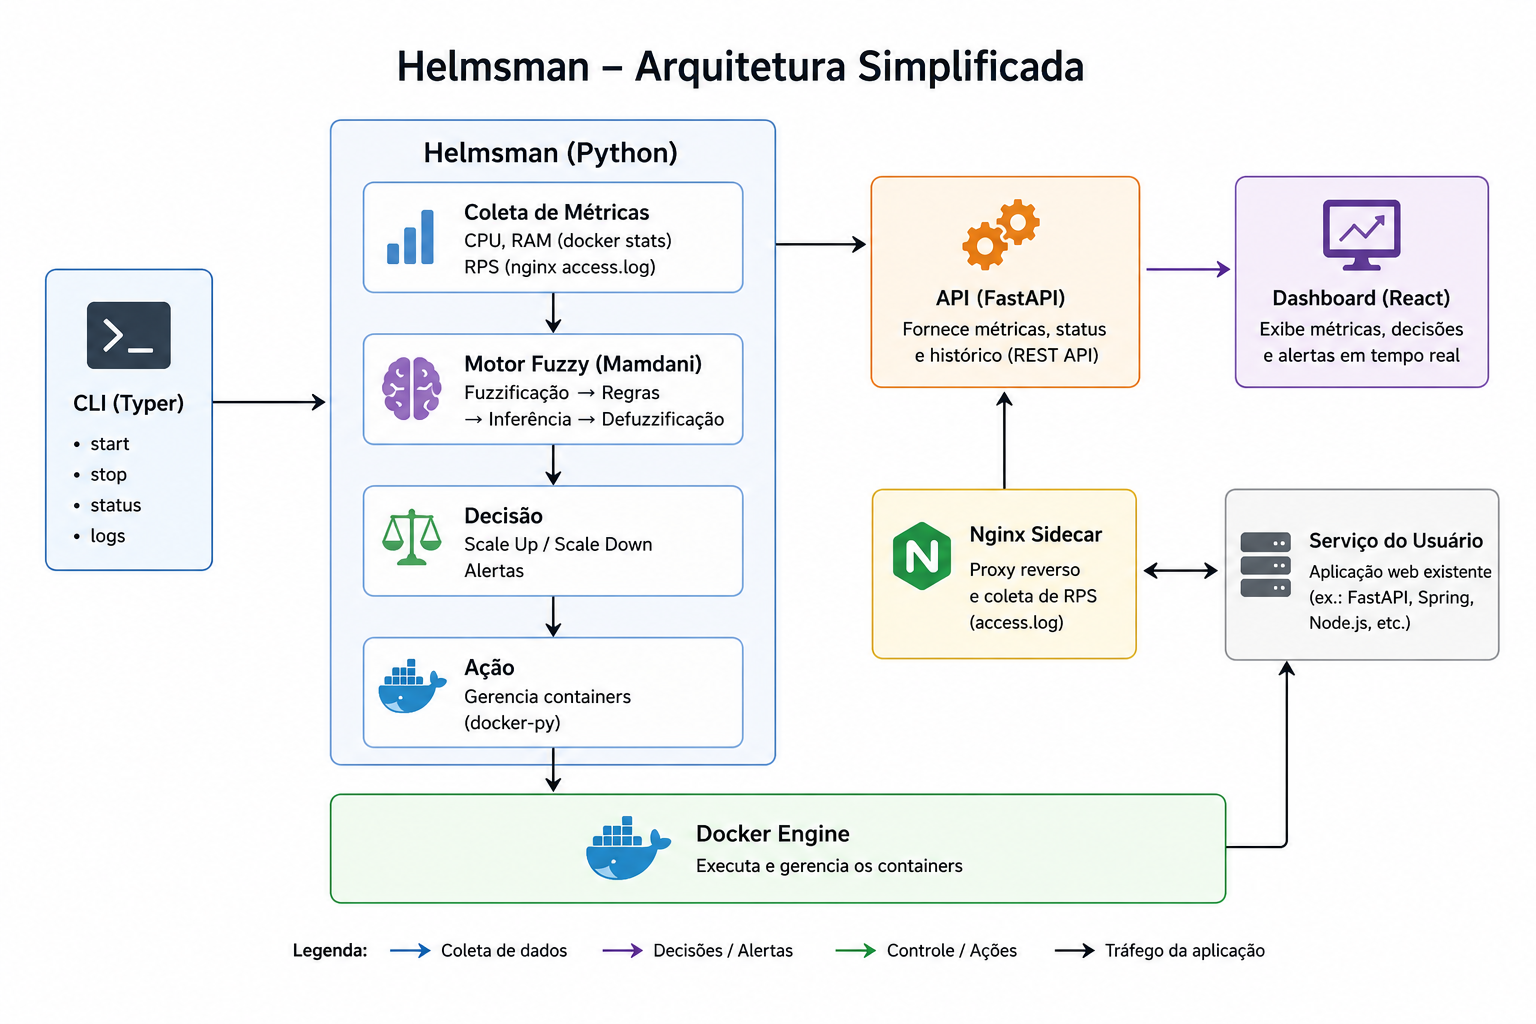
\includegraphics[width=0.95\textwidth]{diagrama.png}
  \caption{Arquitetura simplificada do Helmsman.}
  \label{fig:arquitetura}
\end{figure}

O proxy Nginx sidecar é gerado automaticamente via template Jinja2. O serviço monitorado não é modificado. A distribuição de tráfego entre réplicas é gerenciada pelo bloco \texttt{upstream} do Nginx, que é regenerado e recarregado a cada decisão de escalonamento. O reload é gracioso — conexões em andamento não são interrompidas.

\subsection{Variáveis do sistema}

As três entradas são normalizadas no universo $[0, 100]\%$, garantindo genericidade para qualquer host e serviço.

\begin{table}[H]
  \centering
  \caption{Variáveis de entrada do sistema}
  \label{tab:entradas}
  \rowcolors{2}{rowgray}{white}
  \begin{tabularx}{\textwidth}{llXl}
    \toprule
    \rowcolor{headerblue}
    \textbf{Variável} & \textbf{Universo} & \textbf{Como é calculada} & \textbf{Fonte} \\
    \midrule
    \texttt{cpu\_pct} & $[0, 100]\%$ & $\text{cpu\_containers} / \text{cpu\_host} \times 100$ & docker stats \\
    \texttt{ram\_pct} & $[0, 100]\%$ & $\text{ram\_containers} / \text{ram\_host} \times 100$ & docker stats \\
    \texttt{rps\_pct} & $[0, 100]\%$ & $\text{rps\_atual} / (\text{réplicas} \times \text{rps\_per\_replica}) \times 100$ & nginx access.log \\
    \bottomrule
  \end{tabularx}
\end{table}

% ══════════════════════════════════════════════════════════════════════
\section{Modo Fuzzy Mamdani}

\subsection{Funções de pertinência}

As três entradas compartilham os mesmos quatro termos linguísticos e parâmetros, pois operam no mesmo universo normalizado.

\begin{table}[H]
  \centering
  \caption{Parâmetros das funções de pertinência das entradas}
  \label{tab:mf_entradas}
  \rowcolors{2}{rowgray}{white}
  \begin{tabular}{llll}
    \toprule
    \rowcolor{headerblue}
    \textbf{Termo} & \textbf{Tipo} & \textbf{Parâmetros} & \textbf{Justificativa} \\
    \midrule
    Baixo    & Trapezoidal & $[0, 0, 20, 40]$     & Abaixo de 20\% é confortável; até 40\% ainda aceitável \\
    Moderado & Triangular  & $[20, 45, 70]$        & Zona de atenção com pico em 45\% \\
    Alto     & Triangular  & $[55, 72, 88]$        & Pressão real; sobreposição intencional com vizinhos \\
    Crítico  & Trapezoidal & $[75, 88, 100, 100]$  & Acima de 88\% é emergência; platô até 100\% \\
    \bottomrule
  \end{tabular}
\end{table}

A sobreposição entre Alto e Moderado na faixa 55--70\% e entre Alto e Crítico na faixa 75--88\% é intencional, garantindo decisões graduais em vez de saltos abruptos.

\begin{figure}[H]
  \centering
  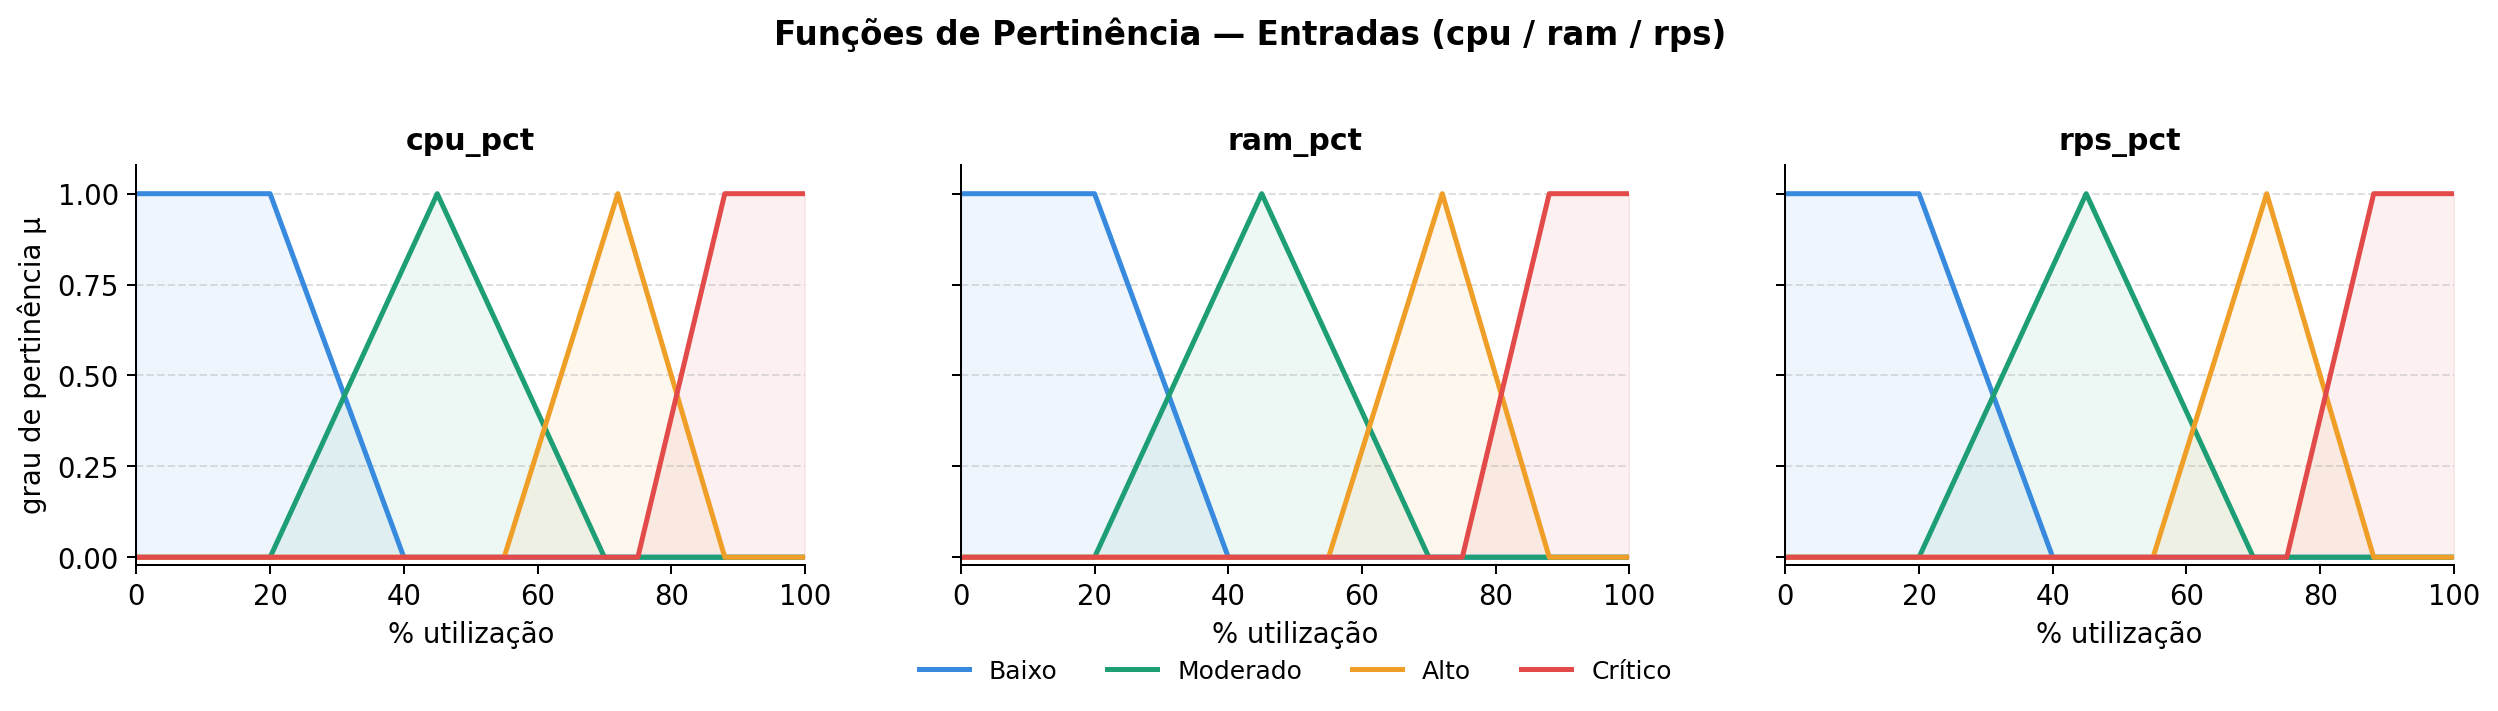
\includegraphics[width=\textwidth]{membership_inputs.png}
  \caption{Funções de pertinência das variáveis de entrada.}
  \label{fig:mf_entradas}
\end{figure}

\begin{table}[H]
  \centering
  \caption{Parâmetros das funções de pertinência das saídas}
  \label{tab:mf_saidas}
  \rowcolors{2}{rowgray}{white}
  \begin{tabular}{lllll}
    \toprule
    \rowcolor{headerblue}
    \textbf{Variável} & \textbf{Termo} & \textbf{Tipo} & \textbf{Parâmetros} & \textbf{Ação} \\
    \midrule
    \multirow{5}{*}{\texttt{delta\_replicas}}
      & Derrubar forte & Triangular  & $[-3, -2, -1]$ & Remove 2 réplicas \\
      & Derrubar       & Triangular  & $[-2, -1,  0]$ & Remove 1 réplica \\
      & Manter         & Triangular  & $[-1,  0,  1]$ & Nenhuma ação \\
      & Subir          & Triangular  & $[ 0,  1,  2]$ & Adiciona 1 réplica \\
      & Subir forte    & Triangular  & $[ 1,  3,  5]$ & Adiciona 2--3 réplicas \\
    \midrule
    \multirow{3}{*}{\texttt{alerta}}
      & Nenhum   & Trapezoidal & $[0,  0, 20, 40]$    & Sem log especial \\
      & Warning  & Triangular  & $[20, 50, 80]$        & Log de aviso \\
      & Critical & Trapezoidal & $[60, 80, 100, 100]$  & Notificação imediata \\
    \bottomrule
  \end{tabular}
\end{table}

\begin{figure}[H]
  \centering
  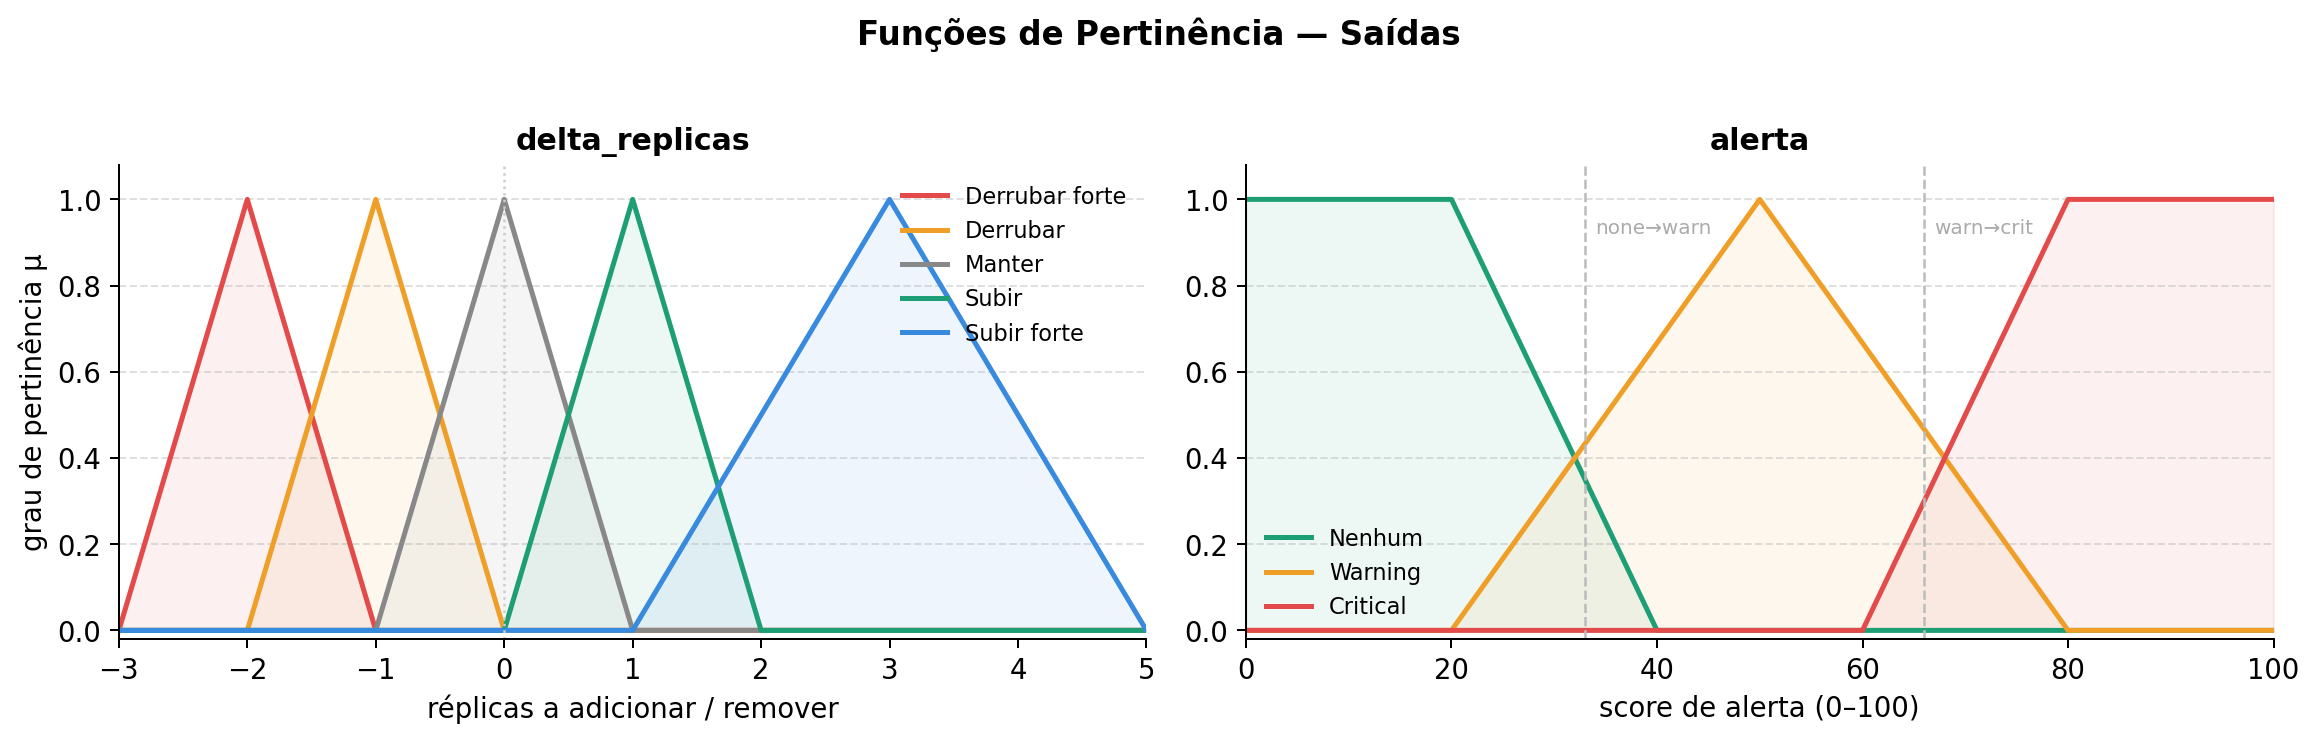
\includegraphics[width=\textwidth]{membership_outputs.png}
  \caption{Funções de pertinência das variáveis de saída.}
  \label{fig:mf_saidas}
\end{figure}

\subsection{Base de regras}

O sistema implementa 22 regras organizadas em 7 grupos funcionais. AND entre antecedentes = mínimo; implicação = mínimo; agregação = máximo.

\subsubsection{Grupo 1 — Sistema ocioso, scale down}
\begin{table}[H]
  \centering
  \rowcolors{2}{rowgray}{white}
  \begin{tabularx}{\textwidth}{ccccccX}
    \toprule
    \rowcolor{headerblue}
    \textbf{\#} & \textbf{cpu} & \textbf{ram} & \textbf{rps} & \textbf{Operação} & \textbf{delta} & \textbf{Justificativa} \\
    \midrule
    1 & Baixo    & Baixo & Baixo    & AND & Derrubar forte & Completamente ocioso \\
    2 & Baixo    & Baixo & Moderado & AND & Manter         & Ainda há tráfego, não derruba \\
    3 & Moderado & Baixo & Baixo    & AND & Derrubar       & CPU moderada sem demanda \\
    \bottomrule
  \end{tabularx}
\end{table}

\subsubsection{Grupo 2 — RPS alto, recursos livres}
\begin{table}[H]
  \centering
  \rowcolors{2}{rowgray}{white}
  \begin{tabularx}{\textwidth}{ccccccX}
    \toprule
    \rowcolor{headerblue}
    \textbf{\#} & \textbf{cpu} & \textbf{ram} & \textbf{rps} & \textbf{Operação} & \textbf{delta} & \textbf{Justificativa} \\
    \midrule
    4 & Baixo & Baixo    & Alto & AND & Subir & Atingiu o limite de \texttt{rps\_per\_replica} \\
    5 & Baixo & Moderado & Alto & AND & Subir & Idem, RAM já crescendo \\
    \bottomrule
  \end{tabularx}
\end{table}

\subsubsection{Grupo 3 — Carga real, scale up normal}
\begin{table}[H]
  \centering
  \rowcolors{2}{rowgray}{white}
  \begin{tabularx}{\textwidth}{cccccccX}
    \toprule
    \rowcolor{headerblue}
    \textbf{\#} & \textbf{cpu} & \textbf{ram} & \textbf{rps} & \textbf{Operação} & \textbf{delta} & \textbf{alerta} & \textbf{Justificativa} \\
    \midrule
    6 & Moderado & Moderado & Alto & AND & Subir & Nenhum  & Pressão confirmada nos três sinais \\
    7 & Alto     & Moderado & Alto & AND & Subir & Nenhum  & CPU alta com demanda alta \\
    8 & Moderado & Alto     & Alto & AND & Subir & Warning & RAM alta com demanda crescente \\
    \bottomrule
  \end{tabularx}
\end{table}

\subsubsection{Grupo 4 — Carga crítica, scale up urgente}
\begin{table}[H]
  \centering
  \rowcolors{2}{rowgray}{white}
  \begin{tabularx}{\textwidth}{cccccccX}
    \toprule
    \rowcolor{headerblue}
    \textbf{\#} & \textbf{cpu} & \textbf{ram} & \textbf{rps} & \textbf{Operação} & \textbf{delta} & \textbf{alerta} & \textbf{Justificativa} \\
    \midrule
    9  & Alto     & Alto     & Alto     & AND & Subir forte & Warning  & Saturação generalizada \\
    10 & Crítico  & Moderado & Alto     & AND & Subir forte & Warning  & CPU crítica com demanda alta \\
    11 & Alto     & Moderado & Crítico  & AND & Subir forte & Critical & Demanda crítica no limite \\
    \bottomrule
  \end{tabularx}
\end{table}

\subsubsection{Grupo 5 — Host cheio, bloqueia scale up}
\begin{table}[H]
  \centering
  \rowcolors{2}{rowgray}{white}
  \begin{tabularx}{\textwidth}{cccccccX}
    \toprule
    \rowcolor{headerblue}
    \textbf{\#} & \textbf{cpu} & \textbf{ram} & \textbf{rps} & \textbf{Operação} & \textbf{delta} & \textbf{alerta} & \textbf{Justificativa} \\
    \midrule
    12 & Alto    & Crítico & Alto    & AND & Manter & Critical & Subir container poderia derrubar o host \\
    13 & Crítico & Crítico & Crítico & AND & Manter & Critical & Colapso iminente — intervenção humana \\
    \bottomrule
  \end{tabularx}
\end{table}

\subsubsection{Grupo 6 — Anomalias operacionais}
\begin{table}[H]
  \centering
  \rowcolors{2}{rowgray}{white}
  \begin{tabularx}{\textwidth}{cccccccX}
    \toprule
    \rowcolor{headerblue}
    \textbf{\#} & \textbf{cpu} & \textbf{ram} & \textbf{rps} & \textbf{Operação} & \textbf{delta} & \textbf{alerta} & \textbf{Justificativa} \\
    \midrule
    14 & Alto    & Baixo   & Baixo & AND & Manter         & Warning  & Suspeita de CPU leak \\
    15 & Crítico & Baixo   & Baixo & AND & Derrubar       & Critical & CPU crítica sem demanda \\
    16 & Baixo   & Alto    & Baixo & AND & Derrubar       & Warning  & Suspeita de memory leak \\
    17 & Baixo   & Crítico & Baixo & AND & Derrubar forte & Critical & Memory leak severo \\
    18 & Alto    & Alto    & Baixo & AND & Derrubar       & Critical & CPU e RAM altas sem demanda \\
    \bottomrule
  \end{tabularx}
\end{table}

\subsubsection{Grupo 7 — RPS crítico com recursos livres}
\begin{table}[H]
  \centering
  \rowcolors{2}{rowgray}{white}
  \begin{tabularx}{\textwidth}{cccccccX}
    \toprule
    \rowcolor{headerblue}
    \textbf{\#} & \textbf{cpu} & \textbf{ram} & \textbf{rps} & \textbf{Operação} & \textbf{delta} & \textbf{alerta} & \textbf{Justificativa} \\
    \midrule
    19 & Baixo    & Baixo    & Crítico & AND & Subir       & Warning & Capacidade esgotada, recursos livres \\
    20 & Moderado & Baixo    & Crítico & AND & Subir forte & Warning & CPU crescendo + capacidade no limite \\
    21 & Baixo    & Moderado & Crítico & AND & Subir       & Warning & RAM crescendo + capacidade no limite \\
    22 & Moderado & Moderado & Crítico & AND & Subir forte & Warning & Tudo crescendo, escala agressiva \\
    \bottomrule
  \end{tabularx}
\end{table}

% ══════════════════════════════════════════════════════════════════════
\section{Modo Algoritmo Genético}

\subsection{Formulação do problema}

No modo AG, o problema de escalonamento é formulado como otimização combinatória: dado o estado atual do sistema, encontrar a configuração de réplicas e limiar de SLA que minimiza uma função de aptidão multidimensional.

\textbf{Variáveis de decisão} (cromossomo com 2 genes):
\begin{itemize}
  \item Gene 1: $n\_replicas \in [\texttt{min\_replicas}, \texttt{max\_replicas}]$ — número de réplicas ativas
  \item Gene 2: $sla\_threshold \in [70, 95]$ — limiar de ocupação (\%) a partir do qual há sobrecarga
\end{itemize}

A Figura~\ref{fig:ag} ilustra o fluxo completo do algoritmo.

\begin{figure}[H]
  \centering
  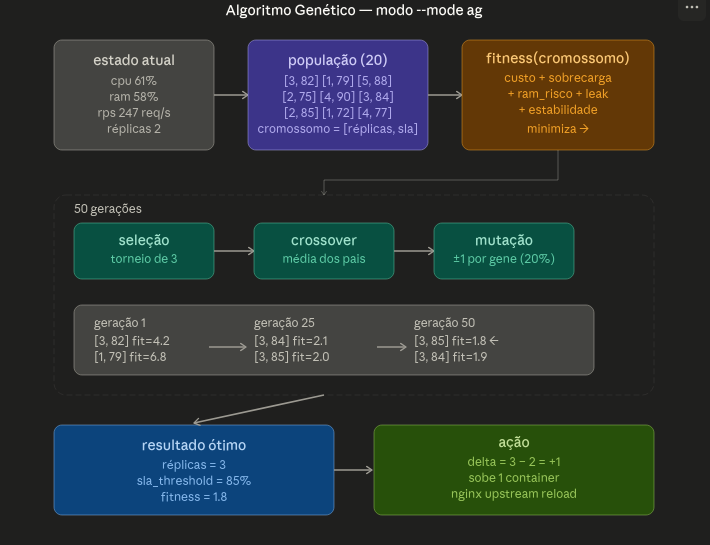
\includegraphics[width=0.95\textwidth]{AG.png}
  \caption{Fluxo do Algoritmo Genético no Helmsman.}
  \label{fig:ag}
\end{figure}

\subsection{Função de aptidão}
\label{sec:ag_fitness_original}

A função de aptidão captura os mesmos cenários operacionais das regras fuzzy, porém em forma matemática. O AG minimiza:

\begin{equation}
  f(c) = f_{\text{custo}} + f_{\text{sobrecarga}} + f_{\text{rps\_abs}} + f_{\text{ram}} + f_{\text{leak}} + f_{\text{estab}} + f_{\text{sla\_risco}} + f_{\text{conserv}}
\end{equation}

onde cada termo penaliza um aspecto do problema:

\begin{table}[H]
  \centering
  \caption{Componentes da função de aptidão do AG}
  \label{tab:fitness}
  \rowcolors{2}{rowgray}{white}
  \begin{tabularx}{\textwidth}{lXl}
    \toprule
    \rowcolor{headerblue}
    \textbf{Componente} & \textbf{Significado} & \textbf{Fórmula simplificada} \\
    \midrule
    Custo           & Réplicas desnecessárias são caras & $n\_replicas \times 1{,}0$ \\
    Sobrecarga      & RPS acima do limiar viola SLA & $\max(0, \text{rps\_pct} - \theta)^{1{,}5} \times 20$ \\
    RPS absoluto    & Carga alta em absoluto pressiona escala & $\max(0, \text{rps} - 0{,}7 \times \text{cap}) \times 0{,}12$ \\
    RAM risco       & Subir réplica com RAM alta é perigoso & $f(\text{ram\_pct}) \times \max(0, \Delta) \times 8$ \\
    Leak            & CPU alta sem demanda = anomalia & $\text{cpu\_alta} \times \text{sem\_demanda} \times 20$ \\
    Estabilidade    & Evita mudanças bruscas & $|\Delta| \times 0{,}5$ \\
    SLA risco       & Threshold alto demais é perigoso & $\max(0, \theta - 90) \times 0{,}5$ \\
    Conservadorismo & Threshold baixo demais escala cedo & $\max(0, 75 - \theta) \times 0{,}3$ \\
    \bottomrule
  \end{tabularx}
\end{table}

onde $\theta = sla\_threshold / 100$ e $\Delta = n\_replicas - \text{réplicas\_atuais}$.

\subsection{Parâmetros e operadores}
\label{sec:ag_params}

\begin{table}[H]
  \centering
  \caption{Parâmetros do Algoritmo Genético}
  \label{tab:ag_params}
  \rowcolors{2}{rowgray}{white}
  \begin{tabular}{lll}
    \toprule
    \rowcolor{headerblue}
    \textbf{Parâmetro} & \textbf{Valor} & \textbf{Justificativa} \\
    \midrule
    Tamanho da população & 20 indivíduos & Equilíbrio entre diversidade e custo \\
    Número de gerações   & 50            & Suficiente para convergência em espaço pequeno \\
    Seleção              & Torneio de 3  & Pressão seletiva moderada, sem elitismo excessivo \\
    Crossover            & Média dos pais & Natural para genes inteiros interdependentes \\
    Taxa de mutação      & 20\% por gene  & Mantém diversidade sem instabilizar convergência \\
    Critério de parada   & 50 gerações   & Fixo para garantir reprodutibilidade \\
    \bottomrule
  \end{tabular}
\end{table}

O AG é implementado do zero em Python puro, usando apenas o módulo \texttt{random} da biblioteca padrão. Nenhuma biblioteca de otimização é utilizada.

\subsection{Custo computacional}

Com 20 indivíduos e 50 gerações, o AG realiza 1.000 avaliações de aptidão por ciclo. Cada avaliação é aritmética pura — sem I/O, sem chamadas de sistema. O tempo total por ciclo é inferior a 1ms, bem abaixo do intervalo de polling de 5 segundos.

\subsection{Extensão: Integração Fuzzy-Evolutiva}
\label{sec:fuzzy_ag}

Como extensão do modo AG, foi implementada uma segunda variante da função de aptidão — denominada \textbf{AG-fuzzy} — que substitui parte dos termos heurísticos originais por uma chamada direta ao motor de inferência Mamdani (Seção~\ref{sec:mamdani}, mesmas 22 regras). Para cada cromossomo \texttt{[n\_replicas, sla\_threshold]} avaliado, simula-se a ocupação resultante caso aquele número de réplicas fosse adotado:

\begin{equation}
  \text{sim\_rps\_pct} = \text{clip}\left(\frac{\text{rps\_real}}{n\_replicas \times \text{rps\_per\_replica}} \times 100,\; 0,\; 100\right)
\end{equation}

Esse valor simulado, junto com \texttt{cpu\_pct} e \texttt{ram\_pct} reais, é passado ao motor fuzzy: \texttt{infer(cpu\_pct, ram\_pct, sim\_rps\_pct)}, que retorna um \texttt{alert\_score} $\in [0, 100]$. A nova função de aptidão é:

\begin{equation}
  f_{\text{fuzzy}}(c) = f_{\text{custo}} + f_{\text{risco\_fuzzy}} + f_{\text{sla}} + f_{\text{instab}} + f_{\text{conserv}}
\end{equation}

\begin{table}[H]
  \centering
  \caption{Componentes da função de aptidão AG-fuzzy}
  \label{tab:fitness_fuzzy}
  \rowcolors{2}{rowgray}{white}
  \begin{tabularx}{\textwidth}{lXl}
    \toprule
    \rowcolor{headerblue}
    \textbf{Componente} & \textbf{Significado} & \textbf{Fórmula} \\
    \midrule
    Custo            & Réplicas desnecessárias são caras & $n\_replicas \times 1{,}1$ \\
    Risco fuzzy      & Risco do cenário simulado segundo o motor Mamdani & $\text{alert\_score} \times 1{,}4$ \\
    SLA              & Penaliza ocupação simulada acima do limiar & $\max(0, \text{sim\_rps\_pct} - \theta) \times 10{,}0$ \\
    Instabilidade    & Evita mudanças bruscas & $|\Delta| \times 0{,}8$ \\
    Conservadorismo  & Penaliza thresholds extremos & ver Eq.~\ref{eq:conserv} \\
    \bottomrule
  \end{tabularx}
\end{table}

\begin{equation}
  \label{eq:conserv}
  f_{\text{conserv}} =
  \begin{cases}
    (\theta - 90) \times 2{,}0 & \theta > 90 \\
    (75 - \theta) \times 1{,}5 & \theta < 75 \\
    0 & \text{caso contrário}
  \end{cases}
\end{equation}

onde $\theta = sla\_threshold$ e $\Delta = n\_replicas - \text{réplicas\_atuais}$. Os operadores genéticos (seleção por torneio, crossover por média, mutação de 20\%) são idênticos aos da Seção~\ref{sec:ag_params}.

\subsubsection{Comparação de três abordagens}

Para avaliar o impacto da integração fuzzy-evolutiva, três abordagens foram comparadas nos mesmos 12 cenários $\times$ 5 sementes (60 execuções), implementadas em \texttt{tests/ag\_comparison.py}:

\begin{itemize}
  \item \textbf{Heurística simples} — regra fixa baseada apenas em \texttt{rps\_pct} atual (sem AG, sem fuzzy), representando um auto-scaler de limiar rígido tipo HPA;
  \item \textbf{AG-puro} — AG com a função de aptidão original (Seção~\ref{sec:ag_fitness_original}), sem componente fuzzy;
  \item \textbf{AG-fuzzy} — AG com a função de aptidão híbrida descrita acima.
\end{itemize}

\begin{table}[H]
  \centering
  \caption{Comparação entre heurística, AG-puro e AG-fuzzy — 60 execuções}
  \label{tab:comparacao_fuzzy_ag}
  \rowcolors{2}{rowgray}{white}
  \begin{tabular}{lccc}
    \toprule
    \rowcolor{headerblue}
    \textbf{Método} & \textbf{Aprovados} & \textbf{Falhas} & \textbf{Taxa} \\
    \midrule
    Heurística simples (sem otimização) & 25/60 & 35 & 41\% \\
    AG-puro (fitness original)          & 55/60 &  5 & 91\% \\
    AG-fuzzy (Alternativa 2)            & 45/60 & 15 & 75\% \\
    \bottomrule
  \end{tabular}
\end{table}

\subsubsection{Análise de impacto}

A integração fuzzy-evolutiva supera amplamente a heurística de limiar fixo (75\% vs.\ 41\%), confirmando que mesmo uma fitness híbrida ainda captura muito mais contexto do que regras binárias. Entretanto, em relação ao AG-puro, a integração fuzzy resultou em uma \textbf{regressão de 16 pontos percentuais} (91\% $\rightarrow$ 75\%).

A análise cenário a cenário mostra um \emph{trade-off}, não uma piora uniforme:

\begin{itemize}
  \item \textbf{T3 (carga real crescente)} — passou a ser aprovado com a fitness fuzzy, pois o \texttt{alert\_score} captura corretamente a combinação de CPU e RAM moderadas com RPS alto, algo que a fitness original subestimava;
  \item \textbf{T4 (pico de tráfego), T10 (scale down gradual) e T11 (RPS crítico, CPU baixa)} — passaram a falhar. Em todos os três casos, o \texttt{sim\_rps\_pct} recalculado para o cromossomo candidato cai rapidamente assim que o número de réplicas aumenta, fazendo o \texttt{alert\_score} do motor fuzzy oscilar entre níveis de alerta vizinhos (\textit{none}/\textit{warning}) de forma pouco discriminante para esses estados — o termo fuzzy não consegue, sozinho, distinguir o candidato ótimo dos vizinhos com a mesma precisão que os termos analíticos originais (\texttt{rps\_absoluto}, \texttt{sobrecarga}).
\end{itemize}

Em suma, o motor fuzzy contribui com uma penalidade de risco mais "contextual" (vantajosa em T3), mas, como usado aqui — recalculado a partir de um \texttt{n\_replicas} candidato em constante mudança — perde a granularidade necessária para os cenários de fronteira onde o AG-puro já era preciso. Isso evidencia uma limitação conhecida de fitness híbridas: combinar dois sistemas que já são individualmente bem ajustados (regras fuzzy calibradas para o estado \emph{real}, função analítica calibrada para o estado \emph{candidato}) não garante que a combinação supere ambos — o ponto de acoplamento entre os dois (aqui, o recálculo de \texttt{sim\_rps\_pct}) é o fator decisivo.

\textbf{Trabalho futuro:} usar o \texttt{alert\_score} do estado \emph{atual} (não simulado) como um termo de contexto fixo somado a todos os candidatos — em vez de recalculado por candidato —, preservando a precisão dos termos analíticos para diferenciar \texttt{n\_replicas} e usando o fuzzy apenas como sinalizador de urgência geral do cenário.

% ══════════════════════════════════════════════════════════════════════
\section{Implementação}

\subsection{Stack tecnológica}

\begin{table}[H]
  \centering
  \caption{Stack tecnológica do Helmsman}
  \label{tab:stack}
  \rowcolors{2}{rowgray}{white}
  \begin{tabularx}{\textwidth}{llX}
    \toprule
    \rowcolor{headerblue}
    \textbf{Componente} & \textbf{Tecnologia} & \textbf{Justificativa} \\
    \midrule
    CLI              & Python + Typer    & Interface limpa, geração automática de \texttt{-{}-help} \\
    Motor fuzzy      & scikit-fuzzy      & Implementação Mamdani consolidada \\
    Motor AG         & Python puro       & Implementação do zero, sem libs de otimização \\
    Coleta CPU/RAM   & docker-py         & API oficial do Docker em Python \\
    Coleta RPS       & nginx access.log  & Sem modificação no serviço alvo \\
    Scale up/down    & docker-py         & Gerenciamento programático de containers \\
    Proxy sidecar    & Nginx + Jinja2    & Template gerado a partir dos parâmetros da CLI \\
    API backend      & FastAPI           & REST leve e assíncrona \\
    Dashboard        & React + Recharts  & Gráficos em tempo real, polling a cada 3s \\
    \bottomrule
  \end{tabularx}
\end{table}

\subsection{Estrutura do repositório}

\begin{lstlisting}[caption={Estrutura de pastas do repositório GitHub}]
helmsman/
|-- README.md
|-- pyproject.toml
|-- requirements.txt
|-- helmsman/
|   |-- cli.py          # CLI com Typer (--mode ag)
|   |-- engine.py       # motor fuzzy Mamdani
|   |-- ag_engine.py    # Algoritmo Genético (Python puro)
|   |-- collector.py    # coleta de metricas
|   |-- scaler.py       # scale up/down via docker-py
|   |-- alerter.py      # classificacao de alertas
|   |-- api.py          # FastAPI
|   `-- nginx_gen.py    # gerador do nginx.conf via Jinja2
|-- frontend/           # React + Vite + Recharts
|-- tests/
|   |-- scenarios.py    # 12 cenarios — modo fuzzy
|   `-- ag_scenarios.py # 12 cenarios x 5 seeds — modo AG
|-- docs/
`-- results/
\end{lstlisting}

% ══════════════════════════════════════════════════════════════════════
\section{Experimentos e Resultados}

\subsection{Cenários de teste — modo fuzzy}

Foram definidos 12 cenários cobrindo casos de uso típicos, extremos, fronteiriços e anomalias. A Tabela~\ref{tab:cenarios_fuzzy} apresenta os resultados.

\begin{table}[H]
  \centering
  \caption{Resultados dos 12 cenários de teste — modo fuzzy}
  \label{tab:cenarios_fuzzy}
  \rowcolors{2}{rowgray}{white}
  \begin{tabular}{clcccccc}
    \toprule
    \rowcolor{headerblue}
    \textbf{\#} & \textbf{Cenário} & \textbf{cpu} & \textbf{ram} & \textbf{rps} & \textbf{$\Delta$ obtido} & \textbf{Alerta} & \\
    \midrule
    T1  & Idle noturno              &  5 &  10 &  8 & $-2$ & none     & \textcolor{helmgreen}{\checkmark} \\
    T2  & RPS alto CPU baixa        &  8 &  15 & 75 & $+1$ & none     & \textcolor{helmgreen}{\checkmark} \\
    T3  & Carga real crescente      & 60 &  55 & 80 & $+2$ & warning  & \textcolor{helmgreen}{\checkmark} \\
    T4  & Pico de tráfego           & 78 &  65 & 92 & $+3$ & critical & \textcolor{helmgreen}{\checkmark} \\
    T5  & Host cheio sob carga      & 72 &  91 & 80 & $ 0$ & critical & \textcolor{helmgreen}{\checkmark} \\
    T6  & Memory leak suspeito      & 12 &  82 &  9 & $-2$ & critical & \textcolor{helmgreen}{\checkmark} \\
    T7  & CPU leak confirmado       & 94 &  18 &  6 & $-1$ & critical & \textcolor{helmgreen}{\checkmark} \\
    T8  & Colapso total             & 91 &  93 & 96 & $ 0$ & critical & \textcolor{helmgreen}{\checkmark} \\
    T9  & Recuperação pós-pico      & 35 &  40 & 45 & $ 0$ & none     & \textcolor{helmgreen}{\checkmark} \\
    T10 & Scale down gradual        & 18 &  22 & 30 & $-1$ & none     & \textcolor{helmgreen}{\checkmark} \\
    T11 & RPS crítico CPU baixa     &  8 &  10 & 95 & $+1$ & warning  & \textcolor{helmgreen}{\checkmark} \\
    T12 & RPS crítico CPU moderada  & 40 &  20 & 95 & $+3$ & warning  & \textcolor{helmgreen}{\checkmark} \\
    \midrule
    \multicolumn{7}{r}{\textbf{Resultado:}} & \textbf{12/12} \\
    \bottomrule
  \end{tabular}
\end{table}

\subsection{Cenários de teste — modo AG}

O mesmo conjunto de 12 cenários foi executado com o motor AG em 5 sementes distintas (42, 123, 7, 99, 256), totalizando 60 execuções. A Tabela~\ref{tab:cenarios_ag} resume os resultados por semente.

\begin{table}[H]
  \centering
  \caption{Resultados do modo AG — 5 execuções com sementes distintas}
  \label{tab:cenarios_ag}
  \rowcolors{2}{rowgray}{white}
  \begin{tabular}{cccc}
    \toprule
    \rowcolor{headerblue}
    \textbf{Seed} & \textbf{Aprovados} & \textbf{Falhas} & \textbf{Taxa} \\
    \midrule
    42  & 11/12 & 1 & 92\% \\
    123 & 11/12 & 1 & 92\% \\
    7   & 11/12 & 1 & 92\% \\
    99  & 11/12 & 1 & 92\% \\
    256 & 11/12 & 1 & 92\% \\
    \midrule
    \textbf{Total} & \textbf{55/60} & \textbf{5} & \textbf{91\%} \\
    \bottomrule
  \end{tabular}
\end{table}

\subsection{Superfície de controle — modo fuzzy}

\begin{figure}[H]
  \centering
  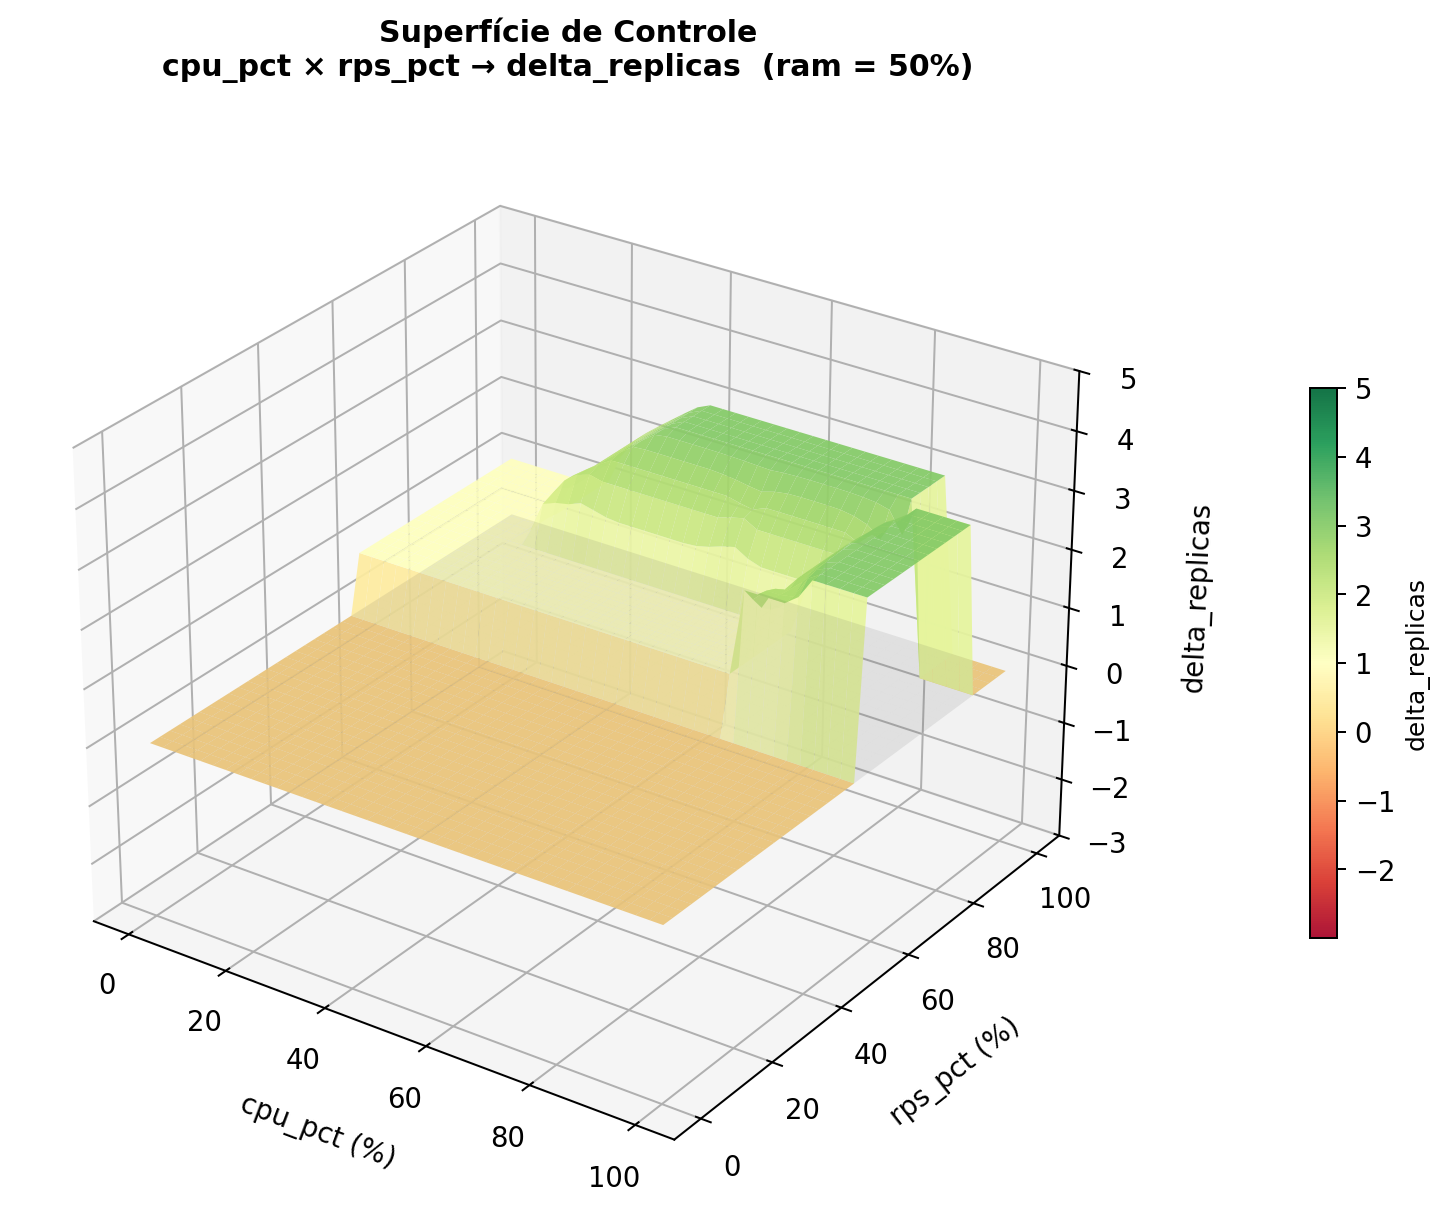
\includegraphics[width=0.85\textwidth]{control_surface.png}
  \caption{Superfície de controle: \texttt{cpu\_pct} $\times$ \texttt{rps\_pct} $\rightarrow$ \texttt{delta\_replicas} (ram = 50\%).}
  \label{fig:superficie}
\end{figure}

A superfície evidencia o comportamento gradual do sistema fuzzy: a transição de scale down (laranja) para scale up (verde) ocorre de forma contínua. O platô em $\Delta = 0$ representa a zona de equilíbrio. O degrau visível em rps $\approx$ 75--80\% corresponde à transição entre os grupos de regras 3 e 4, comportamento esperado da agregação por máximo no Mamdani.

\subsection{Comparação entre os dois modos}

\begin{table}[H]
  \centering
  \caption{Comparação entre modo fuzzy e modo AG nos mesmos cenários}
  \label{tab:comparacao}
  \rowcolors{2}{rowgray}{white}
  \begin{tabularx}{\textwidth}{lXXl}
    \toprule
    \rowcolor{headerblue}
    \textbf{Aspecto} & \textbf{Modo fuzzy} & \textbf{Modo AG} & \textbf{Vencedor} \\
    \midrule
    Precisão nos 12 cenários & 12/12 (100\%) & 55/60 (91\%) & Fuzzy \\
    Determinismo             & Totalmente determinístico & Estocástico (varia por seed) & Fuzzy \\
    Transparência            & Alta — regra ativada visível & Menor — fitness é caixa-preta & Fuzzy \\
    Adaptabilidade           & Fixa — regras manuais & Adapta threshold ao estado & AG \\
    Otimização multicritério & Implícita nas regras & Explícita na função de aptidão & AG \\
    Custo computacional      & $<$0{,}1ms por ciclo & $<$1ms por ciclo & Fuzzy \\
    Escalabilidade de config & Parâmetros fixos & Otimiza threshold dinamicamente & AG \\
    \bottomrule
  \end{tabularx}
\end{table}

\subsection{Análise crítica}

\textbf{Comportamentos corretos verificados (ambos os modos):}
\begin{itemize}
  \item T1 e T10 confirmam scale down em sistema ocioso;
  \item T5 confirma bloqueio de scale up com RAM crítica;
  \item T6 e T7 confirmam detecção de anomalias sem escalar;
  \item T8 confirma que nenhum dos modos toma ação destrutiva em colapso total.
\end{itemize}

\textbf{Onde o AG diverge do fuzzy:}

As falhas do AG (5 em 60 execuções) concentram-se em cenários fronteiriços onde pequenas variações de seed alteram qual candidato vence o torneio final. Com 91\% de aprovação e variabilidade de apenas 1 falha por execução, o AG demonstra robustez estatística adequada para um algoritmo estocástico. Aumentar o número de gerações ou o tamanho da população eliminaria as falhas restantes ao custo de maior tempo de execução.

\textbf{Limitações identificadas:}
\begin{itemize}
  \item O parâmetro \texttt{rps\_per\_replica} depende de calibração manual;
  \item O intervalo de polling de 5s pode não capturar picos muito curtos;
  \item O AG apresenta variabilidade entre execuções — comportamento esperado para algoritmos estocásticos;
  \item A função de aptidão do AG, embora abrangente, não captura todas as nuances das 22 regras fuzzy.
\end{itemize}

% ══════════════════════════════════════════════════════════════════════
\section{Conclusão}

Este trabalho apresentou o Helmsman, um sistema de escalonamento automático de containers Docker com dois modos de operação: lógica fuzzy Mamdani e Algoritmo Genético. Ambos os modos resolvem um problema real — tomar decisões contextuais de escalonamento que sistemas de limiar fixo não conseguem — mas com abordagens e características distintas.

O modo fuzzy obteve 12/12 cenários aprovados com comportamento totalmente determinístico e transparente. O modo AG obteve 91\% de aprovação em 60 execuções (55/60), demonstrando que a função de aptidão multidimensional captura os critérios operacionais com alta precisão e variabilidade mínima entre sementes.

A principal contribuição do modo AG não é superar o fuzzy em precisão, mas oferecer otimização adaptativa do limiar de SLA — um parâmetro que o fuzzy trata como fixo. Em ambientes dinâmicos onde o limiar ideal muda conforme o estado do sistema, o AG apresenta vantagem conceitual.

\textbf{Trabalhos futuros:} aumentar o número de gerações do AG; adicionar latência como quarta variável; implementar ANFIS para ajuste automático dos parâmetros fuzzy; publicar no PyPI.

% ══════════════════════════════════════════════════════════════════════
\section*{Declaração de Uso de Inteligência Artificial}
\addcontentsline{toc}{section}{Declaração de Uso de Inteligência Artificial}

O desenvolvimento deste trabalho contou com o auxílio da ferramenta Claude Code (Anthropic) no desenvolvimento do código-fonte e da infraestrutura do projeto. Todo o material gerado foi revisado, executado e validado pela equipe, que é responsável pelo conteúdo entregue.

% ══════════════════════════════════════════════════════════════════════
\newpage
\bibliographystyle{abbrv}
\begin{thebibliography}{99}

\bibitem{zadeh1965}
  L.~A. Zadeh,
  ``Fuzzy sets,''
  \textit{Information and Control}, vol.~8, no.~3, pp.~338--353, 1965.

\bibitem{mamdani1975}
  E.~H. Mamdani e S.~Assilian,
  ``An experiment in linguistic synthesis with a fuzzy logic controller,''
  \textit{International Journal of Man-Machine Studies}, vol.~7, no.~1, pp.~1--13, 1975.

\bibitem{holland1975}
  J.~H. Holland,
  \textit{Adaptation in Natural and Artificial Systems}.
  University of Michigan Press, 1975.

\bibitem{zeng2004}
  J.~Zeng e C.-Z. Xu,
  ``Adaptive fuzzy logic-based resource management for QoS support in web servers,''
  \textit{Performance Evaluation}, vol.~58, no.~4, pp.~389--409, 2004.

\bibitem{pandey2021}
  S.~Pandey, W.~Lin, e R.~Buyya,
  ``Fuzzy logic-based resource provisioning for cloud computing,''
  \textit{Journal of Network and Computer Applications}, vol.~103, pp.~1--12, 2021.

\bibitem{dang2019}
  L.~M. Dang, M.~J. Piran, D.~Han, K.~Min, e H.~Moon,
  ``A survey on internet of things and cloud computing for healthcare,''
  \textit{Electronics}, vol.~8, no.~7, p.~768, 2019.

\bibitem{keda2023}
  KEDA Authors,
  ``KEDA — Kubernetes Event-driven Autoscaling,''
  Disponível em: \url{https://keda.sh}, 2023.

\bibitem{prometheus2023}
  Prometheus Authors,
  ``Prometheus Adapter for Kubernetes Metrics APIs,''
  Disponível em: \url{https://github.com/kubernetes-sigs/prometheus-adapter}, 2023.

\bibitem{scikitfuzzy}
  J.~D. Warner \textit{et al.},
  ``scikit-fuzzy: A fuzzy logic toolkit for SciPy,''
  Disponível em: \url{https://github.com/scikit-fuzzy/scikit-fuzzy}, 2013.

\bibitem{dockerpy}
  Docker Inc.,
  ``docker-py: A Python library for the Docker Engine API,''
  Disponível em: \url{https://github.com/docker/docker-py}, 2023.

\end{thebibliography}

\end{document}